\documentclass{report}
%\usepackage[utf8]{inputenc}
\usepackage{fontspec} 
\setmainfont{Bookman Old Style} % Times New Roman 
\setsansfont{Tahoma}
\setmonofont{Comic Mono}  
%\setmathfont{Latin Modern Math}
\usepackage[fontsize = 12pt]{fontsize} 
\usepackage{microtype} % added
\usepackage[english, ukrainian]{babel}
\usepackage[
    top = 40pt,
    bottom = 20pt,
    right = 50pt,
    left = 50pt,
    footskip = 15pt,
    %showframe
]{geometry}
\usepackage{amsthm}
\usepackage{amsfonts}
\usepackage{graphicx}
\usepackage[ruled]{algorithm2e}
\usepackage[unicode,
bookmarks = true,
]{hyperref} % edited
\hypersetup{
    colorlinks = true, % edited
    linkcolor = [RGB]{255, 3, 209},
    breaklinks = true,	
    filecolor = magenta,
    citecolor = green,
    anchorcolor = black,
    urlcolor = cyan,
}
\usepackage{biblatex}
\usepackage{csquotes}
\usepackage{mathtools} % {amsmath} already included here
\usepackage{amssymb}
\usepackage{enumitem} % added
\usepackage{nicefrac} % added
\usepackage{tabularray} % added
\usepackage[x11names]{xcolor}
\usepackage{tikz}
\usetikzlibrary{patterns.meta} % added
\usetikzlibrary{decorations.pathmorphing}
\usetikzlibrary {arrows.meta} % added
\usetikzlibrary{calc} % added
\usetikzlibrary{shapes.geometric} % added
\usetikzlibrary{intersections}  % added
\usepackage{pgfplots} % added
\usepackage{pgfplotstable} % added
\pgfplotsset{compat=newest} % added
\usetikzlibrary{pgfplots.fillbetween} % added
\pgfdeclarelayer{pre main} % added
\usepackage{xparse} % added for using \NewDocumentCommand (but not necessary)
\usepackage{rotating} % added
\usepackage{diagbox} % added
\usepackage[center]{caption} % added
\usepackage[warnings-off={mathtools-colon,mathtools-overbracket}]{unicode-math} % added
\usepackage{multirow} % added
\usepackage{fancyhdr} % added
\usepackage[absolute,overlay]{textpos} % added

\begin{document}
\thispagestyle{empty}
\linespread{1.1}

\begin{center}
    {\bfseries\large
        НАЦІОНАЛЬНИЙ ТЕХНІЧНИЙ УНІВЕРСИТЕТ УКРАЇНИ \\
        <<КИЇВСЬКИЙ ПОЛІТЕХНІЧНИЙ ІНСТИТУТ \\
        імені Ігоря СІКОРСЬКОГО>> \\
        Навчально-науковий фізико-технічний інститут \\
        \medskip
        Кафедра математичних методів захисту інформації}
\end{center}

\begin{center}
\vspace{40mm}
{\bfseries\huge Звіт до} \\
{\bfseries\Large комп'ютерного практикуму \No 3} \\
\end{center}

\vspace{55mm}
\begin{center}
    \hfill
    \begin{minipage}[t]{0.4\textwidth}
        \begin{flushright}
            \textbf{Оформлення звіту:} \\ 
            Дигас Богдан, ФІ-52мн \\
            Юрчук Олексій, ФІ-52мн 
        \end{flushright}
    \end{minipage}
\end{center}

\vfill
\begin{center}
    \today \\
    {м. Київ}
\end{center}

\newpage
\pagenumbering{gobble}

\renewcommand{\chaptername}{Комп'ютерний практикум \No}
\makeatletter
\renewcommand{\@pnumwidth}{2em}
\renewcommand{\@tocrmarg}{3em}
\makeatother

\cleardoublepage
\pagenumbering{arabic}
\setcounter{page}{1}
\newpage

% Clear the header and footer
\fancyhead{}
\fancyfoot{}
% Set the right side of the footer to be the page number
\renewcommand{\headrulewidth}{0pt}
\renewcommand{\footrulewidth}{0pt}
\fancyfoot[C]{
  \begin{textblock*}{2cm}(20cm,27.3cm) % bottom right corner of A4
    \small\thepage
  \end{textblock*}
}
\pagestyle{fancy}


\theoremstyle{plain}
\newtheorem{definition}{Означення}%[section]
\newtheorem{theorem}{Теорема}[chapter]
\newtheorem{claim}{Твердження}[chapter]

\theoremstyle{definition}
\newtheorem*{remark}{Зауваження:}
\newtheorem*{example}{Приклад}
\newtheorem{lemma}{Лема}[chapter] 

\renewcommand*{\proofname}{Доведення:} 

\NewDocumentCommand{\MakeWaveComment}{m}{
  \ifmmode % if math mode, make indent before bigger
    \hspace{3pt}
  \fi
  \tikz[baseline={(textnode.base)}]{
    \draw[decorate, decoration={snake, segment length=0.35cm, amplitude=1.5pt}] % Left wave line
    (0,0) -- ++(0,1.5);
    
    \node[anchor=base west, inner sep = 0.5pt] (textnode) at (0.15,0.75) {#1}; % Text node
    
    \draw[decorate, decoration={snake, segment length=0.35cm, amplitude=1.5pt}] % Right wave line
    ([xshift=0.2cm, yshift=-0.75cm]textnode.east) -- ++(0,1.5);
  }
  \ifmmode % if math mode, make indent after bigger
    \hspace{3pt}
  \fi
}

\NewDocumentCommand{\inbuildRef}{mm}{  
  \hyperref[{#1}]{#2}
}

\setcounter{chapter}{2}
\chapter{}
\section{Вступні відомості}
\noindent\textbf{Мета роботи:} Ознайомлення з підходами побудови атак на асиметричні криптосистеми на прикладі атак на криптосистему 
RSA, а саме атаки на основі китайської теореми про лишки, що є успішною при використанні однакового малого значення відкритої експоненти 
для багатьох користувачів та атаки "зустріч посередині"{}, яка можлива у випадку, якщо шифротекст є невеликим числом, що є добутком двох чисел.

\noindent\textbf{Постановка задачі:}
\begin{enumerate}
    \item Створіть репозиторій у системі контролю версій Git/GitHub;
    \item Реалізувати атаку з малою експонентою на основі китайської теореми про лишки.
    \item Реалізувати атаку "зустріч посередині"{} та порівняти її швидкодію з повним перебором можливих відкритих текстів.
    \item Оформити звiт до комп’ютерного практикуму.
\end{enumerate}
\section*{Результати виконання роботи. Варіант 15}

\section{Small exponent attack}
\subsection{Принцип алгоритму:}
Користувач надсилає однакове повідомлення $M$ кільком $k$ користувачам $A_{1}, A_{2}, \dots, A_{k}$, $k \in \mathbb{N}$, 
причому відкритий ключ користувача $A_{i}, i = \overline{1, k}$ -- це пара чисел $(n_{i}, e)$, де $e$ -- деяке мале число. 
Тобто юзери $A_{1}, A_{2}, \dots, A_{k}$ мають однакову експоненту $e$, яка використовується для шифрування. Тоді 
відправник зашифровує своє повідомлення $M$, використовуючи відповідні пари $(n_{i}, e)$ для кожного з отримувачі $A_{i}, i = \overline{1, k}$. 

Зловмисник підключається до каналу передачі даних i перехоплює шифротексти $C_{1}, C_{2}, \dots, C_{k}$, де 
$C_{i} = M^{e} \mod n_{i}, i = \overline{1, k}$ 
Вважаємо, що значення $n_{i}$ для $i = \overline{1, k}$ попарно взаємно прості. (Інакше можна було б обчислити 
$gcd$ i факторизувати, як мінінум, два модуля $n_{i}, n_{j}, i \neq j$, обчислюючи $gcd(n_{i}, n_{j})$). 
А також, що $M < \min\left\{n_{i} \vert i = \overline{1, k}\right\}$. Тобто маємо такий випадок:
\begin{equation*}
    \begin{cases}
        C_{1} = M^{e} \mod n_{1}; \\
        C_{2} = M^{e} \mod n_{2}; \\
        \dots \\
        C_{k} = M^{e} \mod n_{k}. \\
    \end{cases}
\end{equation*}
Якщо $k \geq e$, то зловмисник, перехопивши значення $C_{1}, \dots, C_{k}$, може дешифрувати повідомлення $M$ наступним 
чином:
\begin{enumerate}
    \item Обчислює значення $C = M^{e} \mod \left(n_{1} \cdot n_{2} \cdot \ldots \cdot n_{k}\right)$, 
        використовуючи китайську теорему про лишки;
    \item Оскільки $M < \min\left\{n_{i} \vert i = \overline{1, k}\right\}$, то $M^{e} < n_{1} \cdot n_{2} \cdot \ldots \cdot n_{k}$. 
        Тоді $C = M^{e}$.
    \item Обчислюємо корень $m$-того степеня і знаходимо оригінальне повідомлення: $M = \sqrt[e]{C}$
\end{enumerate}
\subsection{Results of SE}
Згідно варіанту було взято спершу тестовий dummy-варіант, а потім, власне, real завдання. Також для порівняння часу виконання, 
було реалізовано додаткову функцію яка обраховує корені $n$-того степеня методом Ньютона (метод дотичних).

Отримані наступні результати: 
\begin{figure}[!ht]
    \centering
    \begin{minipage}{0.95\linewidth}
        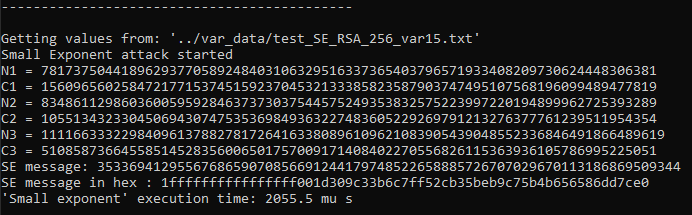
\includegraphics[width=0.95\textwidth, scale=1.2]{ReportPic/report_1_SE_test.png}
    \end{minipage}
    \caption{На тестових даних}
\end{figure}

\begin{figure}[!ht]
    \centering
    \begin{minipage}{0.95\linewidth}
        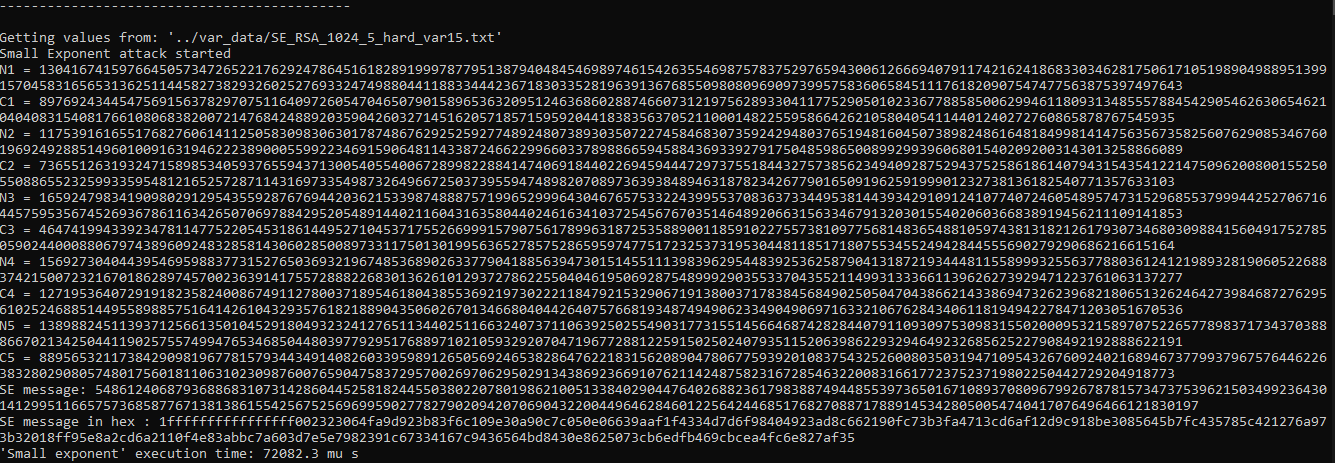
\includegraphics[width=0.95\textwidth, scale=1.5]{ReportPic/report_2_SE_hard_custom.png}
    \end{minipage}
    \caption{На стандартному варіанті, з custom $\sqrt[e]{C}$}
\end{figure}

\newpage % FORCED...
\begin{figure}[!ht]
    \centering
    \begin{minipage}{0.95\linewidth}
        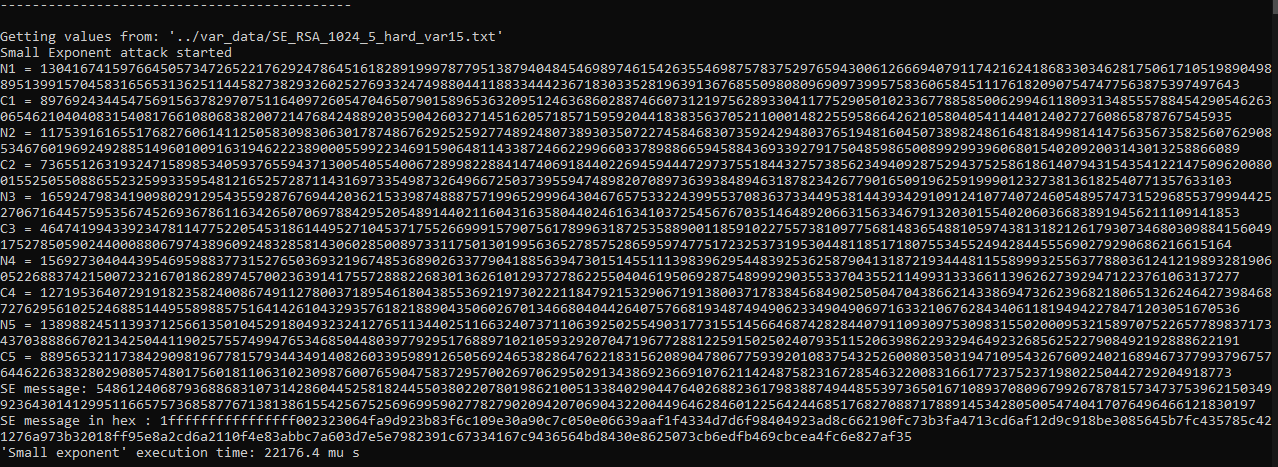
\includegraphics[width=0.95\textwidth, scale=1.5]{ReportPic/report_3_SE_hard_inbuild.png}
    \end{minipage}
    \caption{На стандартному варіанті, з inbuild $\sqrt[e]{C}$}
\end{figure}

Для даного виду атаки, різниця часу у зв'язку з застовуванням іншої функції обчислення $\sqrt[e]{C}$ не є суттєвою, 
вона скаладає $\sim 50000 \, \mu s$, що дорівнює усього $0.05 \, s$. Як можна бачити, стандартна реалізація є більш вдалою. 

\section{Man(Meet) in the middle attack}
\subsection{Принцип алгоритму:}
Зловмисник перехопив деякий шифротекст $C = M^{e} \mod n$, причому відомо, що $M < 2^{l}$, $l \ll \log_{2} n$. 
З доволі великою ймовірністю повідомлення $M$ є складеним числом, тобто його можна представити як добуток чисел 
$M_{1} \cdot M_{2}$. Нехай при цьому $M_{1} \leq 2^{l/2}$ та $M_{2} \leq 2^{l/2}$. Тобто можемо розписати: 
\begin{equation*}
    C = \left(M_{1} \cdot M_{2}\right)^{e} \mod n = M_{1}^{e} \cdot M_{2}^{e} \mod n.
\end{equation*} 
Зловмисник дешифровує повідомлення $M$, виконуючи наступні кроки.
\begin{enumerate}
    \item Криптоаналітик формує множину пар $X$ виду:
        \begin{equation*}
            X = \left\{\left(1, 1\right), \left(2, 2^{e} \mod n\right), \dots, \left(2^{l/2}, \left(2^{l/2}\right)^{e} \mod n\right)\right\}
        \end{equation*}
        Кожна пара має вигляд: $\left(T, T^{e} \mod n\right)$, де $T = \overline{1, 2^{l/2}}$
    \item Далі послідовно обчислює такі значення:
        \begin{equation*}
            C_{S} = C \cdot S^{-e} \mod n, \quad S = \overline{1, 2^{l/2}},
        \end{equation*}
        де $S^{-e} \mod n$ -- попередньо обраховані значення з множини $X$.
        \begin{enumerate}
            \item Для кожного значення $C_{S}$, одразу після його обчислення, зловмисник шукає в множині $X$ 
                таку пару, щоб $S = (T^{e} \mod n)$ для деякого значення $T = \overline{1, 2^{l/2}}$.
            \item Якщо таке $T$ не знайдено, повертаємось на крок 2 та обчислюємо наступне значення $C_{S+1}$. 
                Якщо при цьому $S = 2^{l/2}$, то алгоритм дешифрування зупиняє роботу і виводить \textit{"Відкритий текст 
                не визначено"{}}.
        \end{enumerate}
    \item Для знайденого значення $T^{e} \mod n$ виконується рівність:
        \begin{equation*}
            T^{e} = C \cdot S^{-e} \mod n.
        \end{equation*}
        Тоді маємо:
        \begin{equation*}
            C = \left(T \cdot S\right)^{e} \mod n,
        \end{equation*}    
        тобто шифротекст $C$ було отримано внаслідок шифрування відкритого тексту $T \cdot S$
\end{enumerate}
\subsection{Results of MitM}
Також згідно варіанту було взято тестовий dummy-варіант для MitM, а потім, власне, real завдання. Отримані наступні результати: 

\begin{figure}[!ht]
    \centering
    \begin{minipage}{0.95\linewidth}
        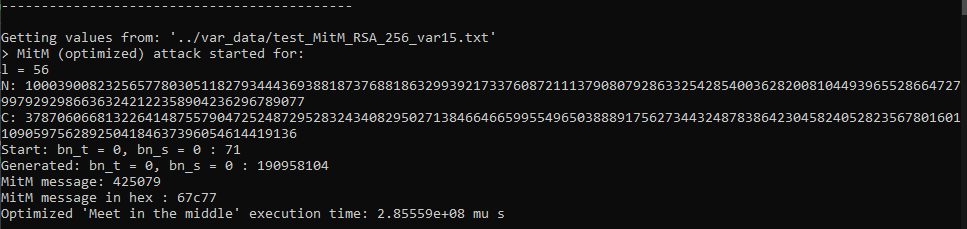
\includegraphics[width=0.95\textwidth, scale=1.5]{ReportPic/report_4_MitM_test.png}
    \end{minipage}
\end{figure}
\begin{figure}[!ht]
    \centering
    \begin{minipage}{0.95\linewidth}
        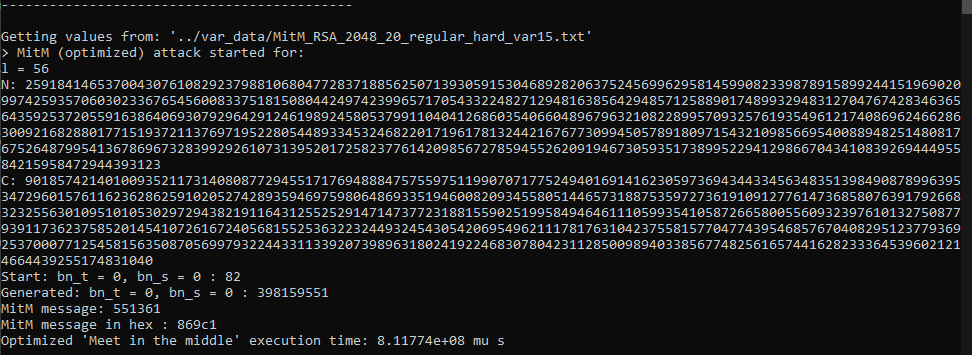
\includegraphics[width=0.95\textwidth, scale=1.5]{ReportPic/report_5_MitM_hard.png}
    \end{minipage}
\end{figure}

Також ми зробили тест bruteforce, який повідомляє час на 1 спробу підбору.
\begin{figure}[!ht]
    \centering
    \begin{minipage}{0.95\linewidth}
        
\includegraphics[width=0.95\textwidth, scale=1.5]{ReportPic/report_6_brutforce_hard.png}
    \end{minipage}
\end{figure}

Помноживши кількість можливих варіантів ключів $2^{2048}$ на $62.6 \, \mu s = 62.6 \times 10^{-6} \, s$ маємо, що час на 
злам прямим перебором займатиме:
\begin{equation*}
    T \approx 2.02 \times 10^{612} \, seconds \approx 6.41 \times 10^{604} \, year
\end{equation*}
Ця цифра є фактично нескінченністю (порівняно з часом життя Всесвіту який дорівнює $1.3798 \times 10^{10} \, year$) для 
будь-яких практичних задач. Навіть за умови надзвичайно оптимізованого паралелізму (використання мільярдів ядерів) 
brutforce 2048-бітного ключа RSA є абсолютно нездійсненним.

\newpage % FORCED...
Далі ми спробували (і змогли!) зробити бонусне завдання додавши оптимізацію. Його результат є наступним:

\begin{figure}[!ht]
    \centering
    \begin{minipage}{0.95\linewidth}
        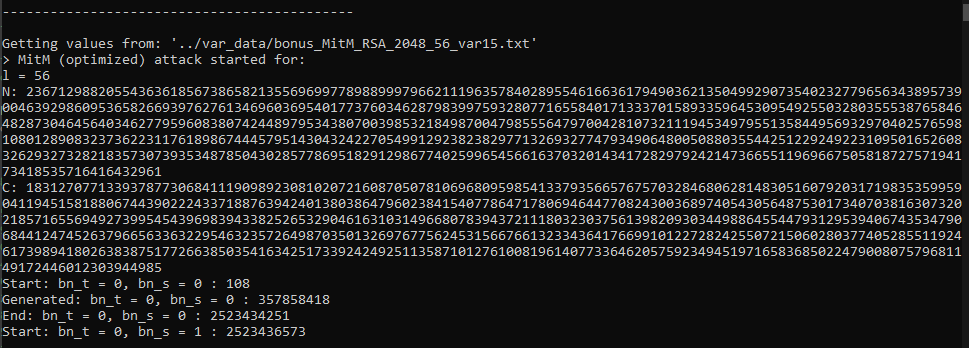
\includegraphics[width=0.95\textwidth, scale=1.5]{ReportPic/report_7_MitM_bonus.png}
    \end{minipage}
\end{figure}

\begin{figure}[!ht]
    \centering
    \begin{minipage}{0.9\linewidth}
        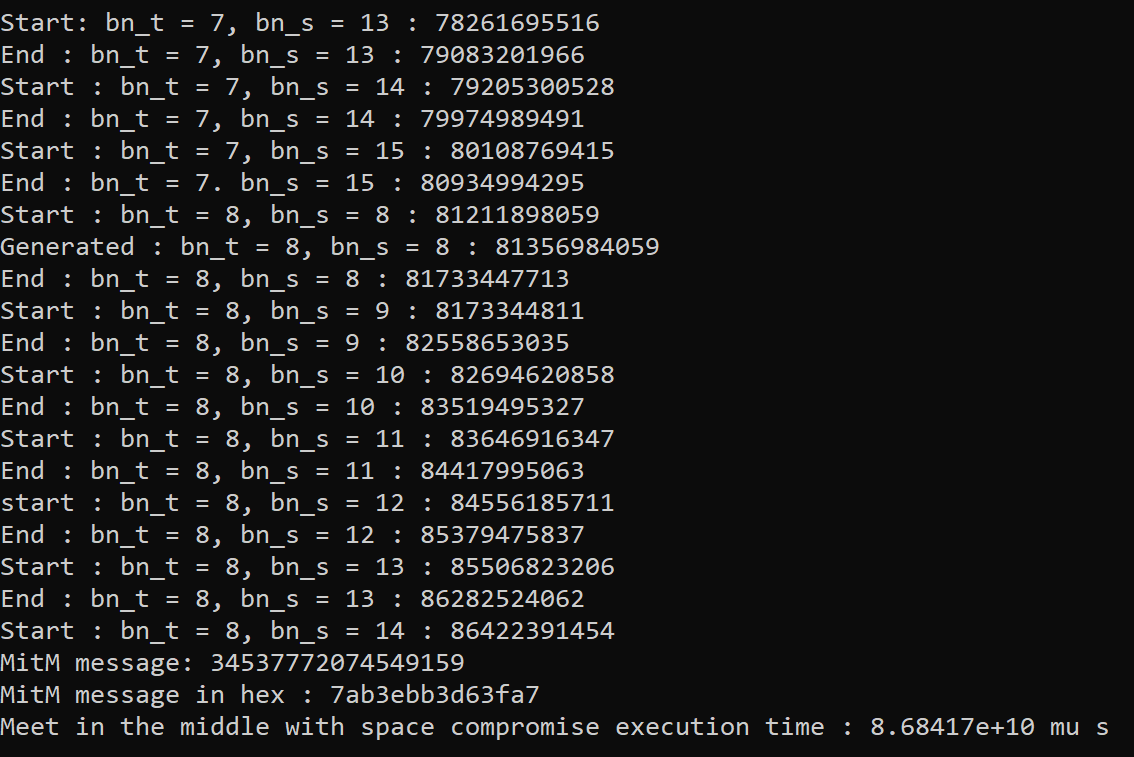
\includegraphics[width=0.90\textwidth, scale=1.2]{ReportPic/report_8_MitM_bonus.png}
    \end{minipage}
\end{figure}

Процес зайняв порядку $24.5$ годин. 

\section{Висновки:}
Завдяки комп'ютерному практикуму ми розібралися з двома атаками на криптосистему RSA, "побачили руками, очами потрогали"{} 
як вони реалізовується на практиці. Було важко розібратися з оптимізацією алгоритму-атаки MitM. За допомогою документації 
C++ ми змогли реалізувати оптимізацію, яка економить ресурси комп'ютера. Довелося робити trade-off крок в бік оптимізації 
під простір і розбити простір перебору на блоки, генерувати їх, очищати, робити перебір і генерувати знову.

Також були думки серіалізувати список $T$, $T^{e} \mod N$, а також були думки з вивантаженням його в постійну пам'ять, 
але нас зупинили думки про I/O overhead та складна програмна реалізація відповідно. Також була ідея з використанням 
іншого API \href{https://arrayfire.org/docs/gettingstarted.htm}{arrayfire} для пришвидшення роботи алгоритму. 

\noindent P.S. На жаль, найбільш наївне рішення проблеми не спрацювало :( \\
\url{https://downloadmoreram.com/}



\end{document}